\section{Task 6 --- Initial Vector (IV) and Common Mistakes}
%
\subsection{IV Experiment}
%

\begin{figure}
    \centering
    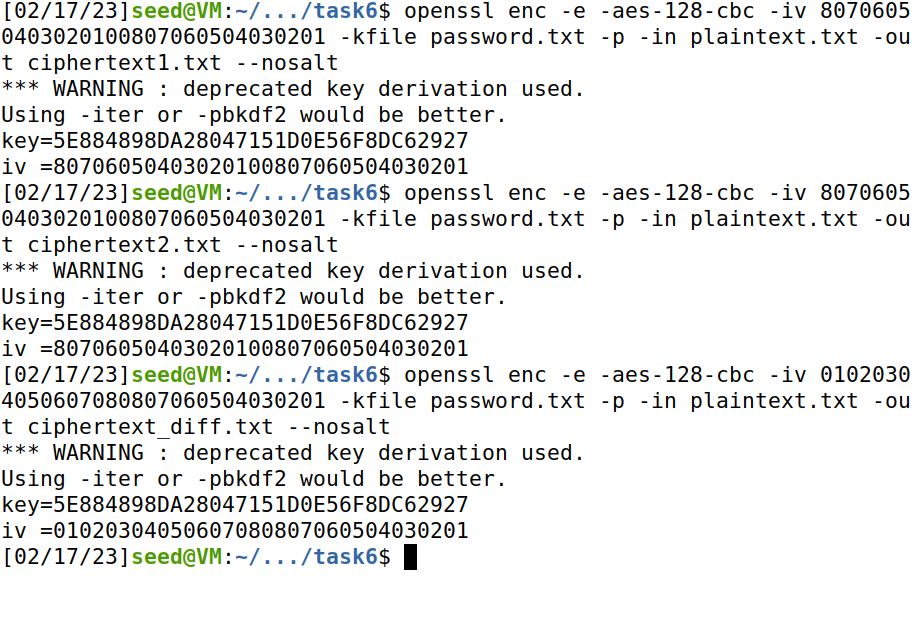
\includegraphics[height=\textheight,width=\textwidth,keepaspectratio]
    {figures/generate_cipher_dif_IV.png}
    \caption{OpenSSL commands to generate ciphertexts.}\label{fig:diff_IV_script}
\end{figure}

\begin{figure}
    \centering
    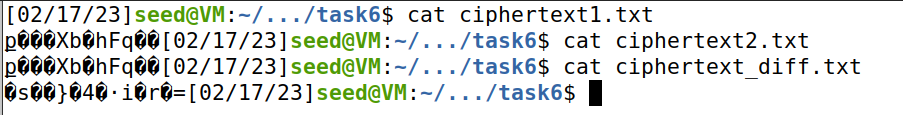
\includegraphics[height=\textheight,width=\textwidth,keepaspectratio]
    {figures/result_diff_IV.png}
    \caption{Resulted ciphertexts with the same and different IVs.}\label{fig:ciphertext_IV}
\end{figure}

The IV we used: {\fontfamily{qcr}\selectfont 80706050403020100807060504030201} for files
{\fontfamily{qcr}\selectfont ciphertext1.txt and ciphertext2.txt}.
IV {\fontfamily{qcr}\selectfont 01020304050607080807060504030201} for
{\fontfamily{qcr}\selectfont ciphertext\_diff.txt} file.

Using the same plaintext.
Identical IVs under same key generates identical ciphertexts.
Diferrent IVs under same key generates different ciphertexts.

\subsection{Common Mistake: Use the Same IV}
%
\begin{lstlisting}[language=Python, caption=A script that finds
    the orginal text P2 (OFB mode).]
#!/usr/bin/python3

# XOR two bytearrays
def xor(first, second):
   return bytearray(x^y for x,y in zip(first, second))

P1   = "This is a known message!"
C1 = "a469b1c502c1cab966965e50425438e1bb1b5f9037a4c159"
C2 = "bf73bcd3509299d566c35b5d450337e1bb175f903fafc159"

# Convert ascii string to bytearray
P1_byte = bytes(P1, 'utf-8')

# Convert hex string to bytearray
C1_byte = bytearray.fromhex(C1)
C2_byte = bytearray.fromhex(C2)

o1 = xor(P1_byte, C1_byte) # output of encryption block | P1 XOR C1
P2_byte = xor(C2_byte, o1) # plaintext of the ciphertext C2

print(str(P2_byte, 'utf-8'))
\end{lstlisting}

\begin{figure}
    \centering
    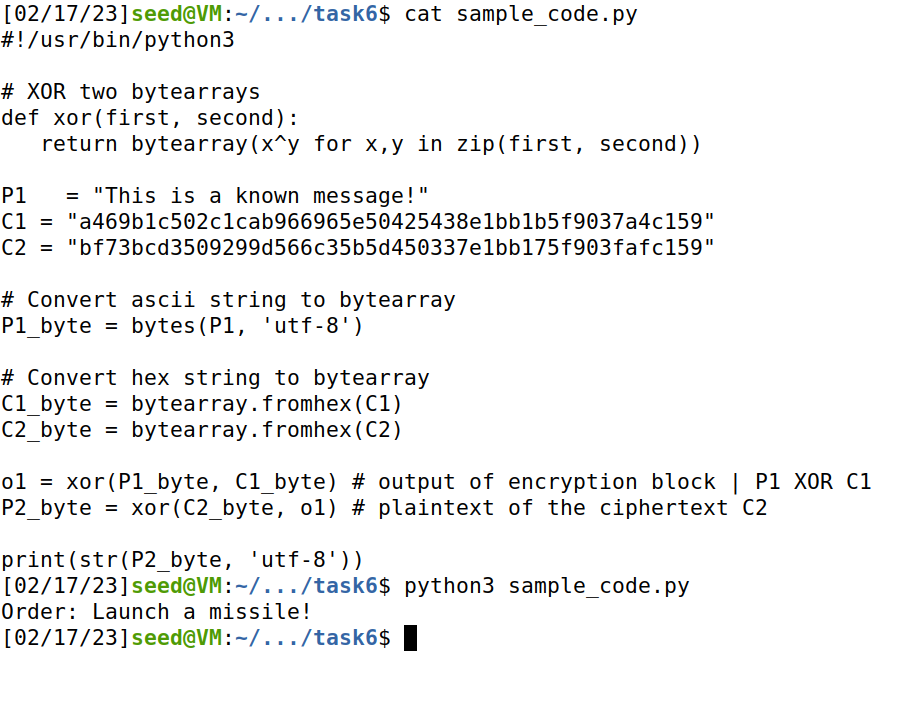
\includegraphics[height=\textheight,width=\textwidth,keepaspectratio]
    {figures/same_IV_OFB.png}
    \caption{Plaintext P2 generated by the Python script.}
    \label{fig:p2_script}
\end{figure}

OFB mode (see \autoref{fig:ofb_dec}).
The plaintext of C2 is
P2: {\fontfamily{qcr}\selectfont Order: Launch a missile!}

CFB mode (see \autoref{fig:cfb_dec}).
only the first block can be reproduced as the same way in OFB mode.

\subsection{Common Mistake: Use a Predictable IV}
%
Look at \autoref{fig:cbc_mode}

Chosen plaintext ``Yes'': {\fontfamily{qcr}\selectfont 5965730d0d0d0d0d0d0d0d0d0d0d0d0d}
Next IV: {\fontfamily{qcr}\selectfont ca43f358cba8d49baac2c91abf0097ac}
IV used: {\fontfamily{qcr}\selectfont d56ac8e4caa8d49baac2c91abf0097ac}

XOR three of above: {\fontfamily{qcr}\selectfont 464c48b10c0d0d0d0d0d0d0d0d0d0d0d}
is also the plaintext need to be fed into the cipher scheme

Ciphertext: {\fontfamily{qcr}\selectfont efdf6fe4b7f660e6abe83a781cff4f9869f04386cc
ba3a039828563e7b9135c6}
Without the padding bytes, it matches the Bob's ciphertext: {\fontfamily{qcr}\selectfont
efdf6fe4b7f660e6abe83a781cff4f98} (see \autoref{fig:chosen_plaintext_attack})

The process above should be mathematically shown

So Bob's secret message is \textbf{Yes}

\begin{figure}
    \centering
    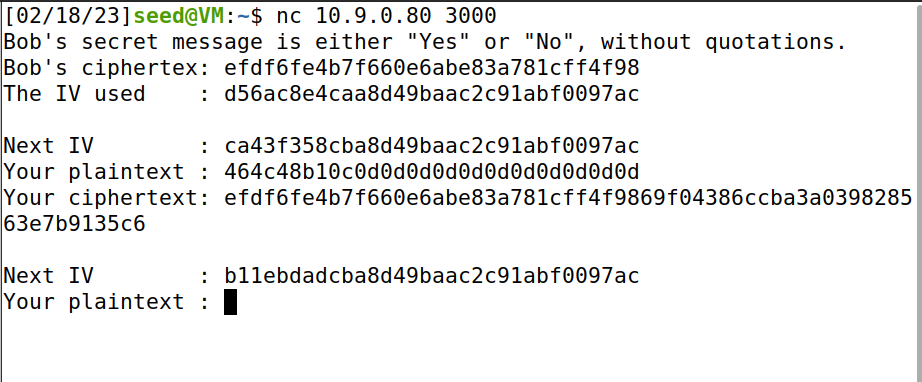
\includegraphics[height=\textheight,width=\textwidth,keepaspectratio]
    {figures/task6_yes.png}
    \caption{Chosen-plaintext attack in the CBC mode.}\label{fig:chosen_plaintext_attack}
\end{figure}